\documentclass[12pt, a4paper]{report}

\usepackage{listings, graphicx, geometry, etoolbox, parskip, caption, subcaption, hyperref, lmodern, minted}
\usepackage{listings}
\usepackage{xcolor}
\usepackage[section]{placeins}
\usepackage[utf8]{inputenc}
\usepackage[T1]{fontenc}
\lstset { %
    language = C,
    backgroundcolor=\color{black!5}, % set backgroundcolor
    basicstyle=\footnotesize,% basic font setting
}
\definecolor{LightGray}{gray}{0.9}
\definecolor{Arsenic}{rgb}{0.1, 0.1, 0.1}
%=================================================================
\makeatletter
% \patchcmd{<cmd>}{<search>}{<replace>}{<success>}{<failure>}
% --- Patch \chapter
\patchcmd{\@makechapterhead}{50\p@}{\chapheadtopskip}{}{}% Space from top of page to CHAPTER X
\patchcmd{\@makechapterhead}{20\p@}{\chapheadsep}{}{}% Space between CHAPTER X and CHAPTER TITLE
\patchcmd{\@makechapterhead}{40\p@}{\chapheadbelowskip}{}{}% Space between CHAPTER TITLE and text
% --- Patch \chapter*
\patchcmd{\@makeschapterhead}{50\p@}{\chapheadtopskip}{}{}% Space from top of page to CHAPTER TITLE
\patchcmd{\@makeschapterhead}{40\p@}{\chapheadbelowskip}{}{}% SPace between CHAPTER TITLE and text
\makeatother
% Set new lengths
\newlength{\chapheadtopskip}\setlength{\chapheadtopskip}{0pt}
\newlength{\chapheadsep}\setlength{\chapheadsep}{10pt}
\newlength{\chapheadbelowskip}\setlength{\chapheadbelowskip}{10pt}

\newgeometry{
    top=2cm,
    bottom=2cm,
    outer=1.5cm,
    inner=1.5cm,
}
%=================================================================

\title{CPS1012 - Tiny Shell Assignment}
\author{Keith Farrugia}
\date{March 2023}

\begin{document}
\maketitle
\newpage
\tableofcontents
\newpage
\chapter{Introduction And Basic Definitions/Concepts}


\section{Introduction}
The following report will explain and describe various aspects and concepts used in creating the Shell. The first part the report will tackle is to explain the basic concepts used throughout the project. Afterwards, it will explain some of the more important algorithms and functions. In terms of explanations the report will loosly follow the sequence of Tasks presented in the assignment specification, but most functions where reworked or improved upon to serve the later tasks that came after.

\section{Basic Definitions}
To facilitate explanations later on, without the need for repetition a basic explanation of how the Shell will handle and categorize input is first needed.

The Shell makes use of a hierarchical set of structures where a given string, usually in the form of the user input, is passed through each of the respective decoders. These act as sieves in order to split said string to its lowest form so that the Shell is able to make use of it.

The struct with the highest level holds the string closest resembling the raw user input is the "Command\_t", The string is then parsed into PipeLine\_t which is in turn further split into Arguments\_t which is finally split into individual arguments (Single\_arg\_t). The figure below (Figure 1.1) should aid in visualizing the explanation of the hierarchy.

\begin{figure}[!htp]
    \centering
    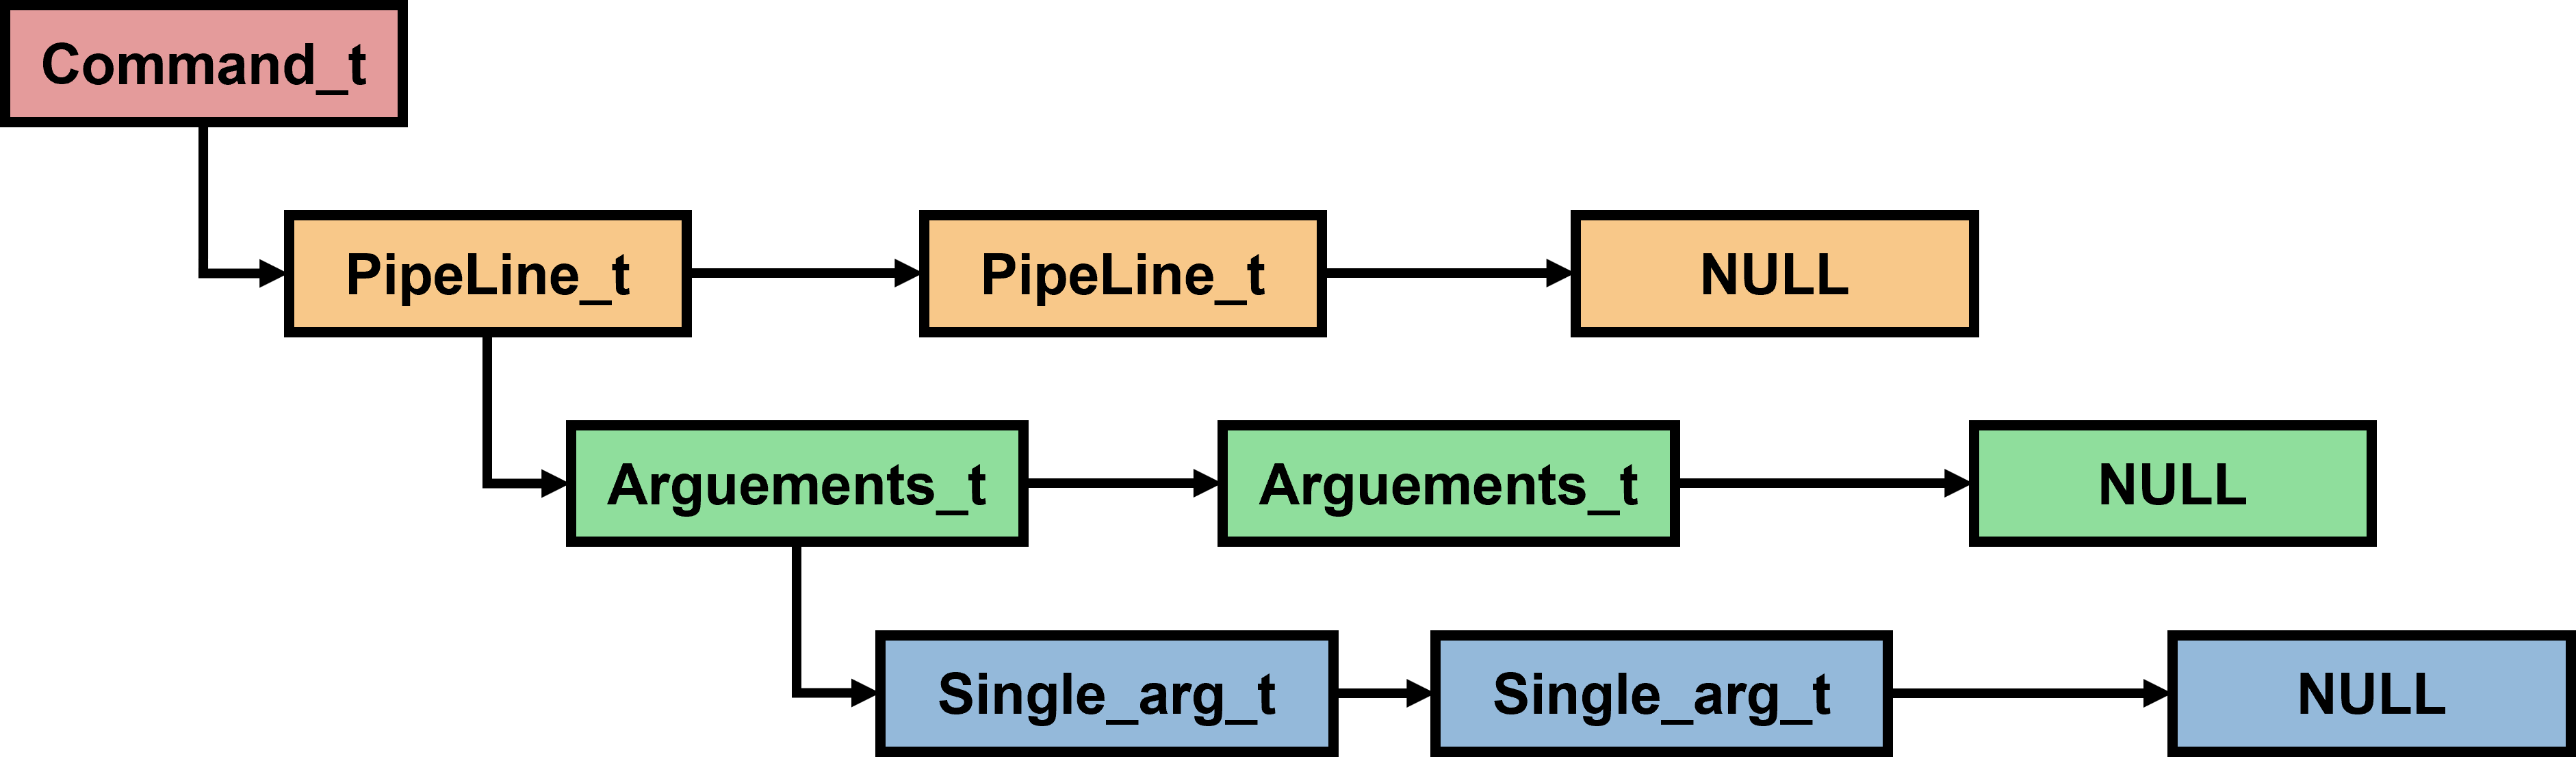
\includegraphics[width=9cm]
    {Diagrams/Structs_Basic.png}
    \caption{Structs Hierarchy}
\end{figure}

As seen in the figure above each layer of struct apart from the Command\_t resembles the form of a linked list serving as a queue. Initially, the program did make use of arrays of pointers (for example char** for the arguments), but this required first parsing a given string in order to count the number of structs that should be malloced and then parsing the string a second time to fill the allocated structs. This firstly, was highly inefficient, and secondly, for task 4, which added more complex character decoding to be taken into consideration, this would prove to complicate the decoding functions since parsing is done twice. Instead, the functions now make use of linked lists where structs can be dynamically allocated and parsing is only done once.

Apart from storing a pointer to a linked list each struct also stores information relative to its stage in the hierarchy, such as the number of elements forming the sub-queue, as well as a pointer to the next element in its hierarchy. The Pipeline\_t struct stores the most information, holding data such as; the file names which input and output should be read or written two as well as whether or not to truncate the output file. It also holds the number of pipes which need to be created to attach its programs together. 

Each level makes use of a metacharacter in order to split the string into substrings. The figure below shows how such a string is split.
\begin{figure}[!htp]
    \centering
    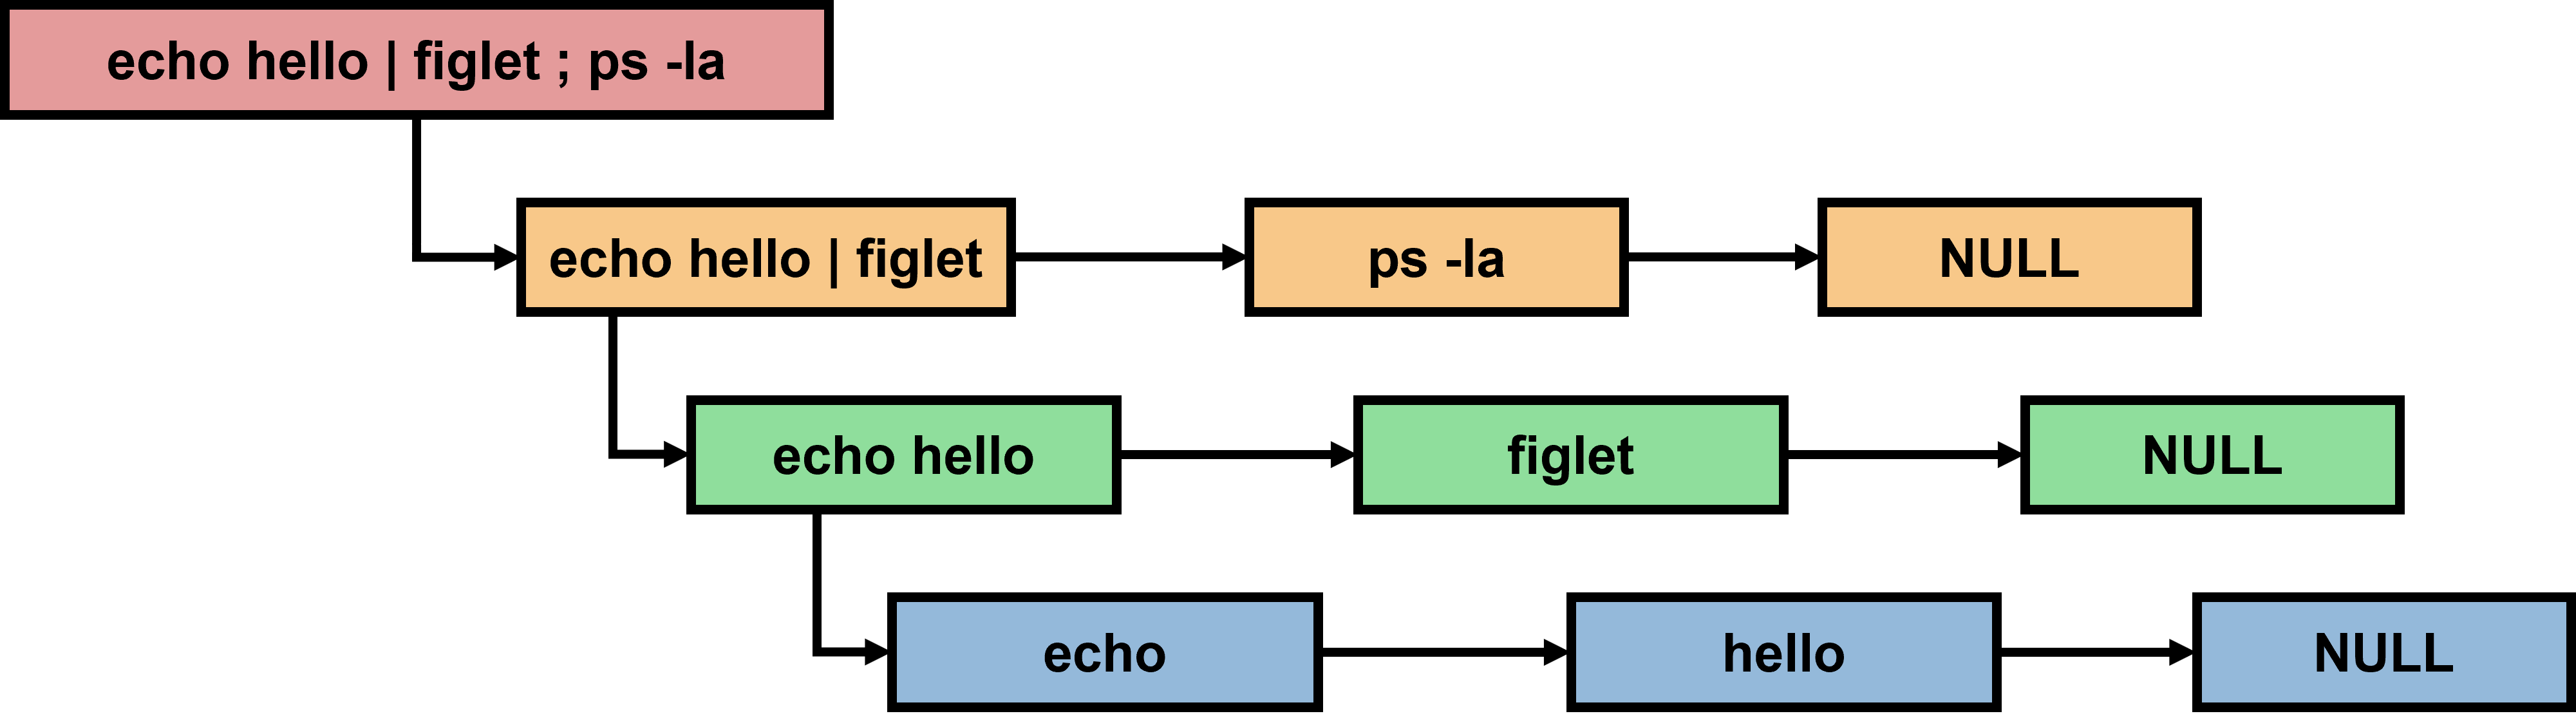
\includegraphics[width=9cm]
    {Diagrams/Structs_Text.png}
    \caption{Example of splitting input}
\end{figure}

The final general struct is that which is used for input validation named execution\_line\_t this struct is used before executing a pipeline in order to validate if said pipeline contains an even number of quotations and if the string includes at least one.

\section{Enums}
Almost all of the functions and methods that will be mentioned in this report make use of an Enum called "ErrorType\_t". This enum holds a list of all possible errors which any function can encounter. The idea behind it was that all a function needs to do when something goes wrong is return the respective error. If the function is called by another function the error simply runs up the chain stopping all processes until it reaches the main method and is handled by the "handleErr" function which prints the required error message. This helps to minimise code repetition.

The second enum set is that of "PipePorts\_t". During the creation of pipes to close either end of the pipe, one needs to specify by either position 0 or 1 of the integer array. This enum aids by making it clearer to understand whether the read or write side of the pipe is being closed.

%================================================================
\chapter{Input Output Redirection}
In order to redirect the input and output of a process as specified by the user, the functions which can be found in the "InputOutputRedirect.c" are used. These will be later mentioned in the "Execute Commands" section. Some of the functions mentioned in this section were constructed similarly to those found in the notes.

\section{file\_exsits()}
This function takes a file name and tries to open said file in order to see if it does in fact exist in the current directory. This is done through a file pointer and the "fopen" function. If the file pointer is NULL then the file does not exist and the function returns false. Else the function closes the file and returns true.

\section{reopen()}
This function takes in 4 parameters, one for the file descriptor to be changed (fd) for example STDIN\_FILENO, another for the path of the file which will replace it (path), and the last two for the flags and modes specified. Making use of dup2, the function first opens the file specified by the path with the passed flags and mods, it then replaces whichever file pointer in the file descriptor table with the newly opened file and closes any unused file pointers. If successful it returns "Success" else it returns the required error.

\section{redirect\_input()}
In order to make use of the previously mentioned function to set the input file of a process, the Shell makes use of this function. It simply takes as an input a file name which it then asks the reopen() function to replace with the STDIN\_FILENO file descriptor.

\section{redirect\_output()}
Similarly, this process replaces STDOUT\_FILENO with whatever file name is passed as a parameter. Additionally, it also asks for a boolean to specify whether the inputted file should be truncated or appended which is then set through the flags. 

%================================================================

\chapter{Execute Commands}
The execute functions are mostly included in the .c file "ExecuteFunctions" and its respective header file. This section will go into detail explaining the core concepts of the methods related to the fork and execute principle as well as that of pipelining. Although this section is closely related to Task 1 of the assignment specifications, many of the methods to be mentioned have been changed in order to be suited to work with the later tasks.

\section{wait\_for\_child()}
The wait\_for\_child(), function isn't overly complicated. Its purpose is to simply wait until the child process indicated by the 'pid' parameter finishes its execution. It returns an ErrorType\_t depending on whether it successfully waited for the child and whether the child has successfully executed. It is mainly called during the last program in a given pipeline so that the parent waits for the pipeline to finish.

\section{fork\_exec()}
This function is the most basic implementation of the fork and execute principle. Taking a list of arguments and a pid pointer to fill with the child pid, the function forks a child and passes the arguments using the execvp function. This function serves no real use in the scope of the shell since its simpling implementation the fork\_exec\_pipe serves as a more robust variant allowing for more customization with its larger capacity of parameters.

\section{fork\_exec\_pipe()}
In addition to the parameters mentioned for the previous function, the fork\_exec\_pipe() also takes pointers to two integer arrays of length 2 which should be used to set the input and output pipes. These should be set in whatever parent function calls this function. Additionally, it also takes 2 strings which are used to set the input and output redirect pipes as well as a boolean in order to specify whether the output should be appended or truncated to the respective file. The function forks a child program this time setting the input and output pipes or setting the redirects using 'dup2' or the redirect input/output functions. If any of these are set to NULL then the child program continues with the default settings. Ultimately, the child program executes whatever program is specified in the parameters. In the case of the parent program, it immediately closes its access to the input pipe in order to prevent issues such as deadlocks.

\section{execute\_pipeline()}
In order to execute a sequence of programs that form a pipeline, this method is called. Making use of the "Pipeline\_t" struct mentioned before, in order to take the pointer to the first program (Arguments\_t), it traverses the linked list creating a child and executing each program making use of the fork\_exec\_pipe(). In order to create the pipes necessary to connect the aforementioned programs, the function creates a 2D array of integers depending on the precalculated number of pipes stored in the "Pipeline\_t" struct. Since the arguments to be passed into the execvp are required to be an array of strings and not a queue, the function Queue\_to\_String() is called which returns an array of pointers to each of the single argument strings effectively creating the array of strings that is required. 

Depending on whether the current program is the first, last or in between of the pipeline the function passes the pipes or redirects necessary. If the program is the first in the pipeline then no input pipe is passed but instead a redirect input file is specified. Similarly, if the program is the last one in the pipeline then the same is done with the output pipe and the redirect output file, the parent also waits for this child to finish if async is set to false. If the program does not meet any of the above cases then an input and output pipe are both specified while neither redirect file is given. If the program is the only one in its pipeline then no pipes are given and only the redirects are specified, the parent also waits for the child if async is false.

The function will call freePipeline() if any errors where met or if the pipeline has finished executing.

%================================================================

\chapter{Builtin Commands}
As specified by Task 2 the Shell also has a set of built-in functions. The code related to this can be found inside the "Builtin.c" and its respective ".h" file. All functions follow the same parameter and return type style set as the "builtin\_t" function type created in the header file. this is so that the function could be added to an array of built-in commands.

\section{builtin\_exit()}
This function is the least complicated of the set and simply exits and ends the shell's execution with the enum EXIT\_SUCCESS.

\section{builtin\_cd()}
This function makes use of the second string in the array in order to change the current working directory. It does so through the "chdir" function and returns whether it has been successful or not.

\section{builtin\_cwd()}
When the user asks for the current working directory the builtin\_cwd function is called. By making use of the "getcwd()" method this process is able to print the current working directory of the shell. The string length is specified by the PATH\_MAX variable which is defined in the "linux/limits" library.

\section{builtin\_ver()}
The builtin\_ver process doesn't affect the shell in a similar manner to the previously mentioned functions. It simply makes use of print lines to show information about the shell for the user and some personal comments.

\section{compare\_builtin()}
The 4 built-in functions explained above were all placed inside an array of structs (builtin\_list) which attaches the string representing the command and its handler function. The compare\_builtin() method takes an array of strings and compares the first string to each of the commands in the builtin\_list array. If a command matches then the handler is called and any errors are handled. If the function finds a matching string it returns true, else it returns false.

%================================================================

\chapter{Decoding Pipes and Arguments}
The following code analysis will go over the functions most closely related to the specifications of task 3. As stated before most of the functions don't only adhere to the requirements set by task 3 but were also changed to match the requirements set by task 4. These functions can be found inside the "DecodePipesAndArgs" '.c' and '.h' files.

\section{validateToken()}
Before executing a given pipeline the shell must first make sure that it is valid, more specifically for the main meta characters, in this case. This is done by the validateToken() function. 

The program will traverse the string representing the pipeline from the start and from the end. If the first character which isn't whitespace happens to be the '|' character which represents a pipe the function will print the appropriate message and return an error. The pipe metacharacter is the only character which is required to not be the first character in an input.

If the first character is not a pipe symbol then the function traverses the array from the end. At the first character from the end of the string which is not a whitespace, the function will loop through the list of tokens ('|', '<', '>') checking if the character is part of that group. If it does the function then check whether it is the '>' since the error message is a bit different to include both the '>' and the '>>' symbols. Either way, the function prints an error message and returns an error.

If the character is not part of the specified meta characters then the function returns Success meaning that the string is valid.

\section{Decode\_Redirect\_out()}
In the case that the user wishes to redirect the output of a program the input will include the '>' meta character. The purpose of this function is to find whether or not the user has inputted this character, and if he has read the file specified.

The first loop is used to traverse the string until it finds the redirect symbol ('>'). The loop checks 3 conditions for each character. If the current character is a backslash ('\textbackslash'), then the function will skip the next two characters, for the second character is cancelled by the backslash and does not need to be checked. If the character is a quotation mark then the program will read all characters up to the next quotation, if any backslash is found it is treated as before. This effectively performs a jump skipping all characters since if the metacharacter being searched is there inside the quotation it is nullified.

If the character is found then the function replaces it with a whitespace, this is so that it is removed from the string and not parsed as an argument later. The next character is then checked if this is also a second redirect symbol (ie the user has inputted '>>') then the function replaces it with another whitespace and the truncate boolean inside the pipeline struct is set to false. If the user has only inputted a single '>' then truncate is set to true. The function then breaks from the loop. If the character meets none of the mentioned conditions, the loop moves to the next character

The second loop is used to read the spaces that might be between the  redirect symbol and the file name, every space is skipped until a non-whitespace character is met and the loop is exited.

The final thing the function needs to do is to actually read the file specified. Here the function follows a similar pattern to before. It will loop through the string from where it left off, if a '\textbackslash' is found the function replaces it with a whitespace and saves the character after. If it finds a quotation mark it saves all characters up to the next quotation. If it finds a whitespace character then it is deemed as the end of the filename and ends the reading of a file. Else it reads the character into the buffer (temp). Any character read are all replaced by whitespace after they are saved inside the buffer 'temp', in order to remove them from the string so that they will not be read as arguments.

If the buffer is not empty, the function replaces the last character with the end-of-line character, mallocs the needed space for the filename, points the pipeline->filname to the allocated memory, and finally copies the string to store it in the malloced area. If no file has been found then the file pointer is set to NULL.

\section{Decode\_Redirect\_in()}
Likewise, the Decode\_Redirect\_in is an almost carbon copy of the redirect-out decoder. The only difference is in the finding of the metacharacter where this time the character to be found is '<' and there is no checking for a double symbol like the '>>'. Apart from that the reading and allocation of the file name are the same.

\section{split\_Program\_into\_Arguments()}
This is the start of the decoding functions and is the last level (in the hierarchy) of decoding. Its purpose is to split a given program into separate arguments. As a visual example, it is what happens between the green and blue stages (Figure 1.2).  In terms of how the algorithm works, it follows very closely to how the decoding works in the Redirect functions. Although this time it repeats itself after saving an argument in order to read the next one.

In order to read one argument the program follows these steps. If the program first finds a space it skips all spaces until a character which isn't a whitespace is found. It then starts reading the argument similarly to how the filename was read before; any backslashes are skipped with the next character automatically read (if it is not out of bounds), any characters after a quotation is read until the next quotation, anything else is read as normal, and finally if a whitespace is met after a non-whitespace character then it is deemed to be the end of the argument. Once an argument has been successfully read it is stored at the end slot of the Single\_arg\_t linked list. The process repeats for the next argument until it reaches the end of the string.

\section{Queue\_to\_String()}
Since the execvp() function only accepts an array of strings, it is not compatible with the current structure of the linked list which holds the separate arguments as strings. It was for this reason that this function was created. By allocating an array of double char pointers (char**), which is the length of the number of arguments + 1, The function traverses the linked list pointing each index of the string array to one of the single arguments. This effectively creates something which is compatible with the execvp() function. The final string in the array is set to NULL.

\section{Display and Free Arguments}
The displayArgList() serves no actual function in the shell and was mostly used in the debugging phase of the project. It prints the list of single arguments as well as the number of arguments. The reason for the tabs is that the function is usually used in tendon with the other display functions hence the indentation serves as a separation between the hierarchy.

The freeArguments() function is used in order to free the allocated variables making up the linked list once the process has finished its job. It traverses the list freeing both the string and the related struct.

\section{split\_PipeLine\_into\_Program}
Taking one step up the hierarchy this function now splits a given command into separate pipes. Using Figure 1.2 as a reference, this will be the conversion from the yellow level that the green. The function makes use of the pipeline struct in order to store the linked list of arguments and other information. For this explanation, the word command will reference a string which can include multiple or no pipes (ex "echo hello | figlet"). A program is a string which lies on either side of a pipe or between two pipes ("echo hello"). The program is later split into arguments using the function split\_Program\_into\_Arguments(), if the argument count is 0 meaning there are no arguments then the program stops and returns an error.

In this case, the function is a lot simpler when it comes to decoding. The only characters not included in the program string are the pipe symbols '|'. Meaning that any other metacharacter or regular character including whitespace is left to be dealt with in the split\_Program\_into\_Arguments() function. 

The function loops through a given string saving all the characters it comes across, similarly to before if a backslash is found the program reads the next space this time also reading the backslash in order to decode it later. If a quotation is found the program reads all the characters up to the next quotation including the quotations themselves. If the function meets a pipe symbol or the end of the string, and the value it has read at least one character, the function creates an Argument\_t struct to add to the end of the pipeline args list and sends the program-filled string to be decoded using the split\_Program\_into\_Arguments() method. Before ending the function also calculates the number of pipes needed using the number of programs.

\section{Free and Display Pipeline}
Correspondingly to the freeArguments() function, there is a need to free; the linked list made of the arguments, other variables such as the file redirects and the PipeLine\_t struct itself. The function freePipeline(), traverses the argument list calling the freeArguments() for each element. It then frees any other variables which are no longer needed.

In addition, the displayPipeline() is another utility function which was used during the debugging phase, displaying all variables saved in the struct as well as the separate arguments with the use of the displayArgList() function.

\chapter{Advanced Scanning}
This section is an explanation connected to the "AdvancedDecode" '.c' and '.h' files. This section is closely related to Task 4 of the assignment specification. However, this is not the only section affected by this task since most of the other decode functions were reworked in order to meet the requirements. Therefore this file was created to hold 2 main functions, one related to decoding commands while the other a validation function related to quotations. The file also includes some utility functions.

\section{validate\_and\_quote\_Sting()}
Before a pipeline can be decoded and executed it is first validated. This validation is separate from the validation done for task 3a. The function makes use of a struct called execution line which holds a string, the number of quotations and if the string is ultimately valid. The function loops through the character of a string checking and counting all the quotations, any backslashes are skipped. It also checks if there is at least one alphanumeric character in the string else there would be nothing to run.

If there is not an even number of quotations or there doesn't exist at least one alphanumeric character then the function sets valid to false and then an error message is printed. The function also checks if the string is NULL.

\section{Decode\_Command()}
The first level of decoding which needs to be done on the user input is to split the string into a list of commands. This function does so by filling the pipeline list in Command\_t with each pipeline the user wants to execute. As a function, it is almost identical to the function split\_PipeLine\_into\_Program() with the only difference being that instead of a pipe symbol the function searches for the end command symbol ';'. The function also doesn't call the next stage of decoding but only stores the string in the pipeline struct.

\section{Utility Functions}
displayStates() is a function used in order to print whether an input is valid or not and was used during the debugging phase.

freeCommandline() traverses the pipeline-linked list deleting only the structs since the pipelines themselves should already have been freed by the execute function.

displayCommands() is used in tandem with the other display commands to show the entire structure and all the commands pipelines and arguments. Again this was only used for debugging.

\chapter{Main Function and Test Cases}

\section{Main Function}
The main function which is executed in order to run the shell, is found in "Shell.c". The main function starts by first taking the user input from Linenoise and decodes it into pipelines using Decode\_Command. The function then for each pipeline; validates the string by quotation and alphanumeric, validates the tokens (metacharacters), and then decodes the redirects and the pipeline taking care of validation. Before the execution starts the function checks if the input file exists, and then decides whether it was a builtin command or not and executes accordingly. This is repeated until there are no more commands in the list and the user input is read again.

\section{Tests}
The following section will show some test cases given to the Shell.

\subsection{Testing Basic Decoding}
Test Cases:
\begin{itemize}
  \item echo "Hello World" > Hello.txt
  \item figlet <Hello.txt
  \item echo Bye | figlet
  \item e"ch"o \textbackslash"Hello\textbackslash"
\end{itemize}
\begin{figure}[!htp]
    \centering
    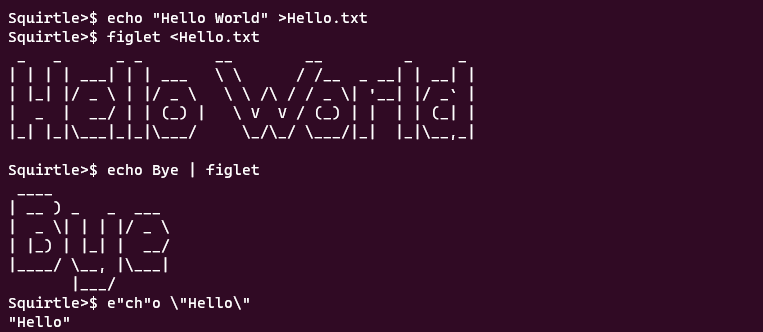
\includegraphics[width=9cm]
    {Diagrams/Shell_Test_1}
    \caption{Test of Basic Decoding}
\end{figure}

\newpage

\subsection{More Advanced Decoding 1}
BUG: The following test is inconsistent and does sometimes create an error related to malloc. 
Test Cases:
\begin{itemize}
  \item echo "This is a list of quoted metacharacters : \textbackslash" < > >> | \textbackslash\textbackslash"  
\end{itemize}
\begin{figure}[!htp]
    \centering
    
\includegraphics[width=9cm]
    {Diagrams/Shell_Test_2}
    \caption{Test of more advanced Decoding}
\end{figure}

\subsection{More Advanced Decoding 2}
Test Cases:
\begin{itemize}
  \item echo "hello" > text.txt; figlet < text.txt >out.txt; cat out.txt 
\end{itemize}
\begin{figure}[!htp]
    \centering
    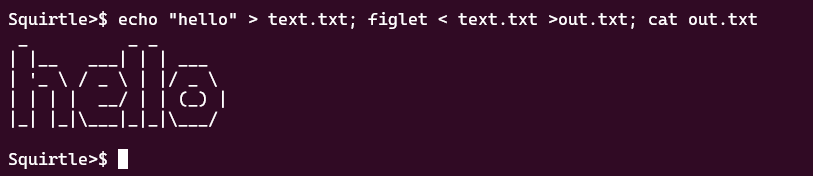
\includegraphics[width=9cm]
    {Diagrams/Shell_Test_5}
    \caption{Test of redirect input and output in unison}
\end{figure}

\subsection{Builtin functions}
Test Cases:
\begin{itemize}
  \item mkdir cps1012; ls; cd cps1012; cwd
\end{itemize}
\begin{figure}[!htp]
    \centering
    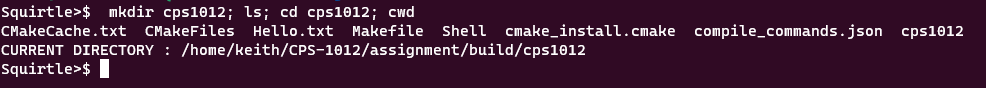
\includegraphics[width=9cm]
    {Diagrams/Shell_Test_3}
    \caption{Test of Builtin functions}
\end{figure}

\subsection{Error Handling}
Test Cases:
\begin{itemize}
  \item a
  \item |
  \item a|
  \item "a
\end{itemize}
\begin{figure}[!htp]
    \centering
    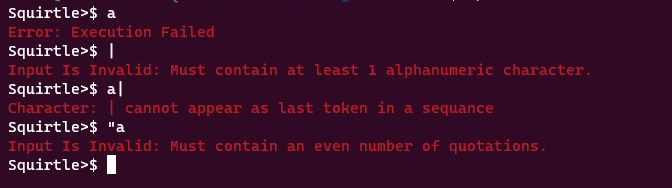
\includegraphics[width=9cm]
    {Diagrams/Shell_Test_4}
    \caption{Error Handling Test}
\end{figure}
\end{document}
